% !TEX root = ../../../thesis.tex
For this sample lateral constriction junctions (ScS)\footnote{Also called a Dayem bridge, see~\cite{likharevSuperconductingWeakLinks1979}.} were used. The advantage is that the behaviour of the junction depends strongly on $\xi$.\cite{likharevSuperconductingWeakLinks1979} As such, due to the temperature dependence of $\xi$ we can tune the junction behaviour. The size of the constriction should ideally be around $3\xi$.\cite{likharevSuperconductingWeakLinks1979}

Our method benefits from a small $\lambda$, as can be seen in our figure of merit (Section~\ref{sec:figure-of-merit}). As such we used \ce{Nb} as our superconductor\footnote{Other candidates were \ce{NbTi} and \ce{MoGe}, they however have a much larger penetration depth.}. At \qty{0}{\kelvin} \ce{Nb} has $\lambda = \qty{47}{\nano\meter}$ and $\xi = \qty{38}{\nano\meter}$.\cite{maxfieldSuperconductingPenetrationDepth1965}

The fabrication followed the method outlined in Section~\ref{sec:method-sample-fabrication}. Due to a machine malfunction \qty{113}{\nano\meter} of \ce{Nb}\footnote{This was measured using an Atomic Force Microscope (AFM) by M. Westerdijk.} was deposited. The target thickness was \qty{90}{\nano\meter}. The fine structures made using the FIB, can be seen in Figure~\ref{fig:CP1.2H-SEM-images}. The geometries of the sample can be found in Table~\ref{tab:CP1.6H-geometries}.

\begin{figure}[ht!]
	\begin{subfigure}[t]{0.3\textwidth}
		\centering
		\def\svgwidth{\textwidth}
		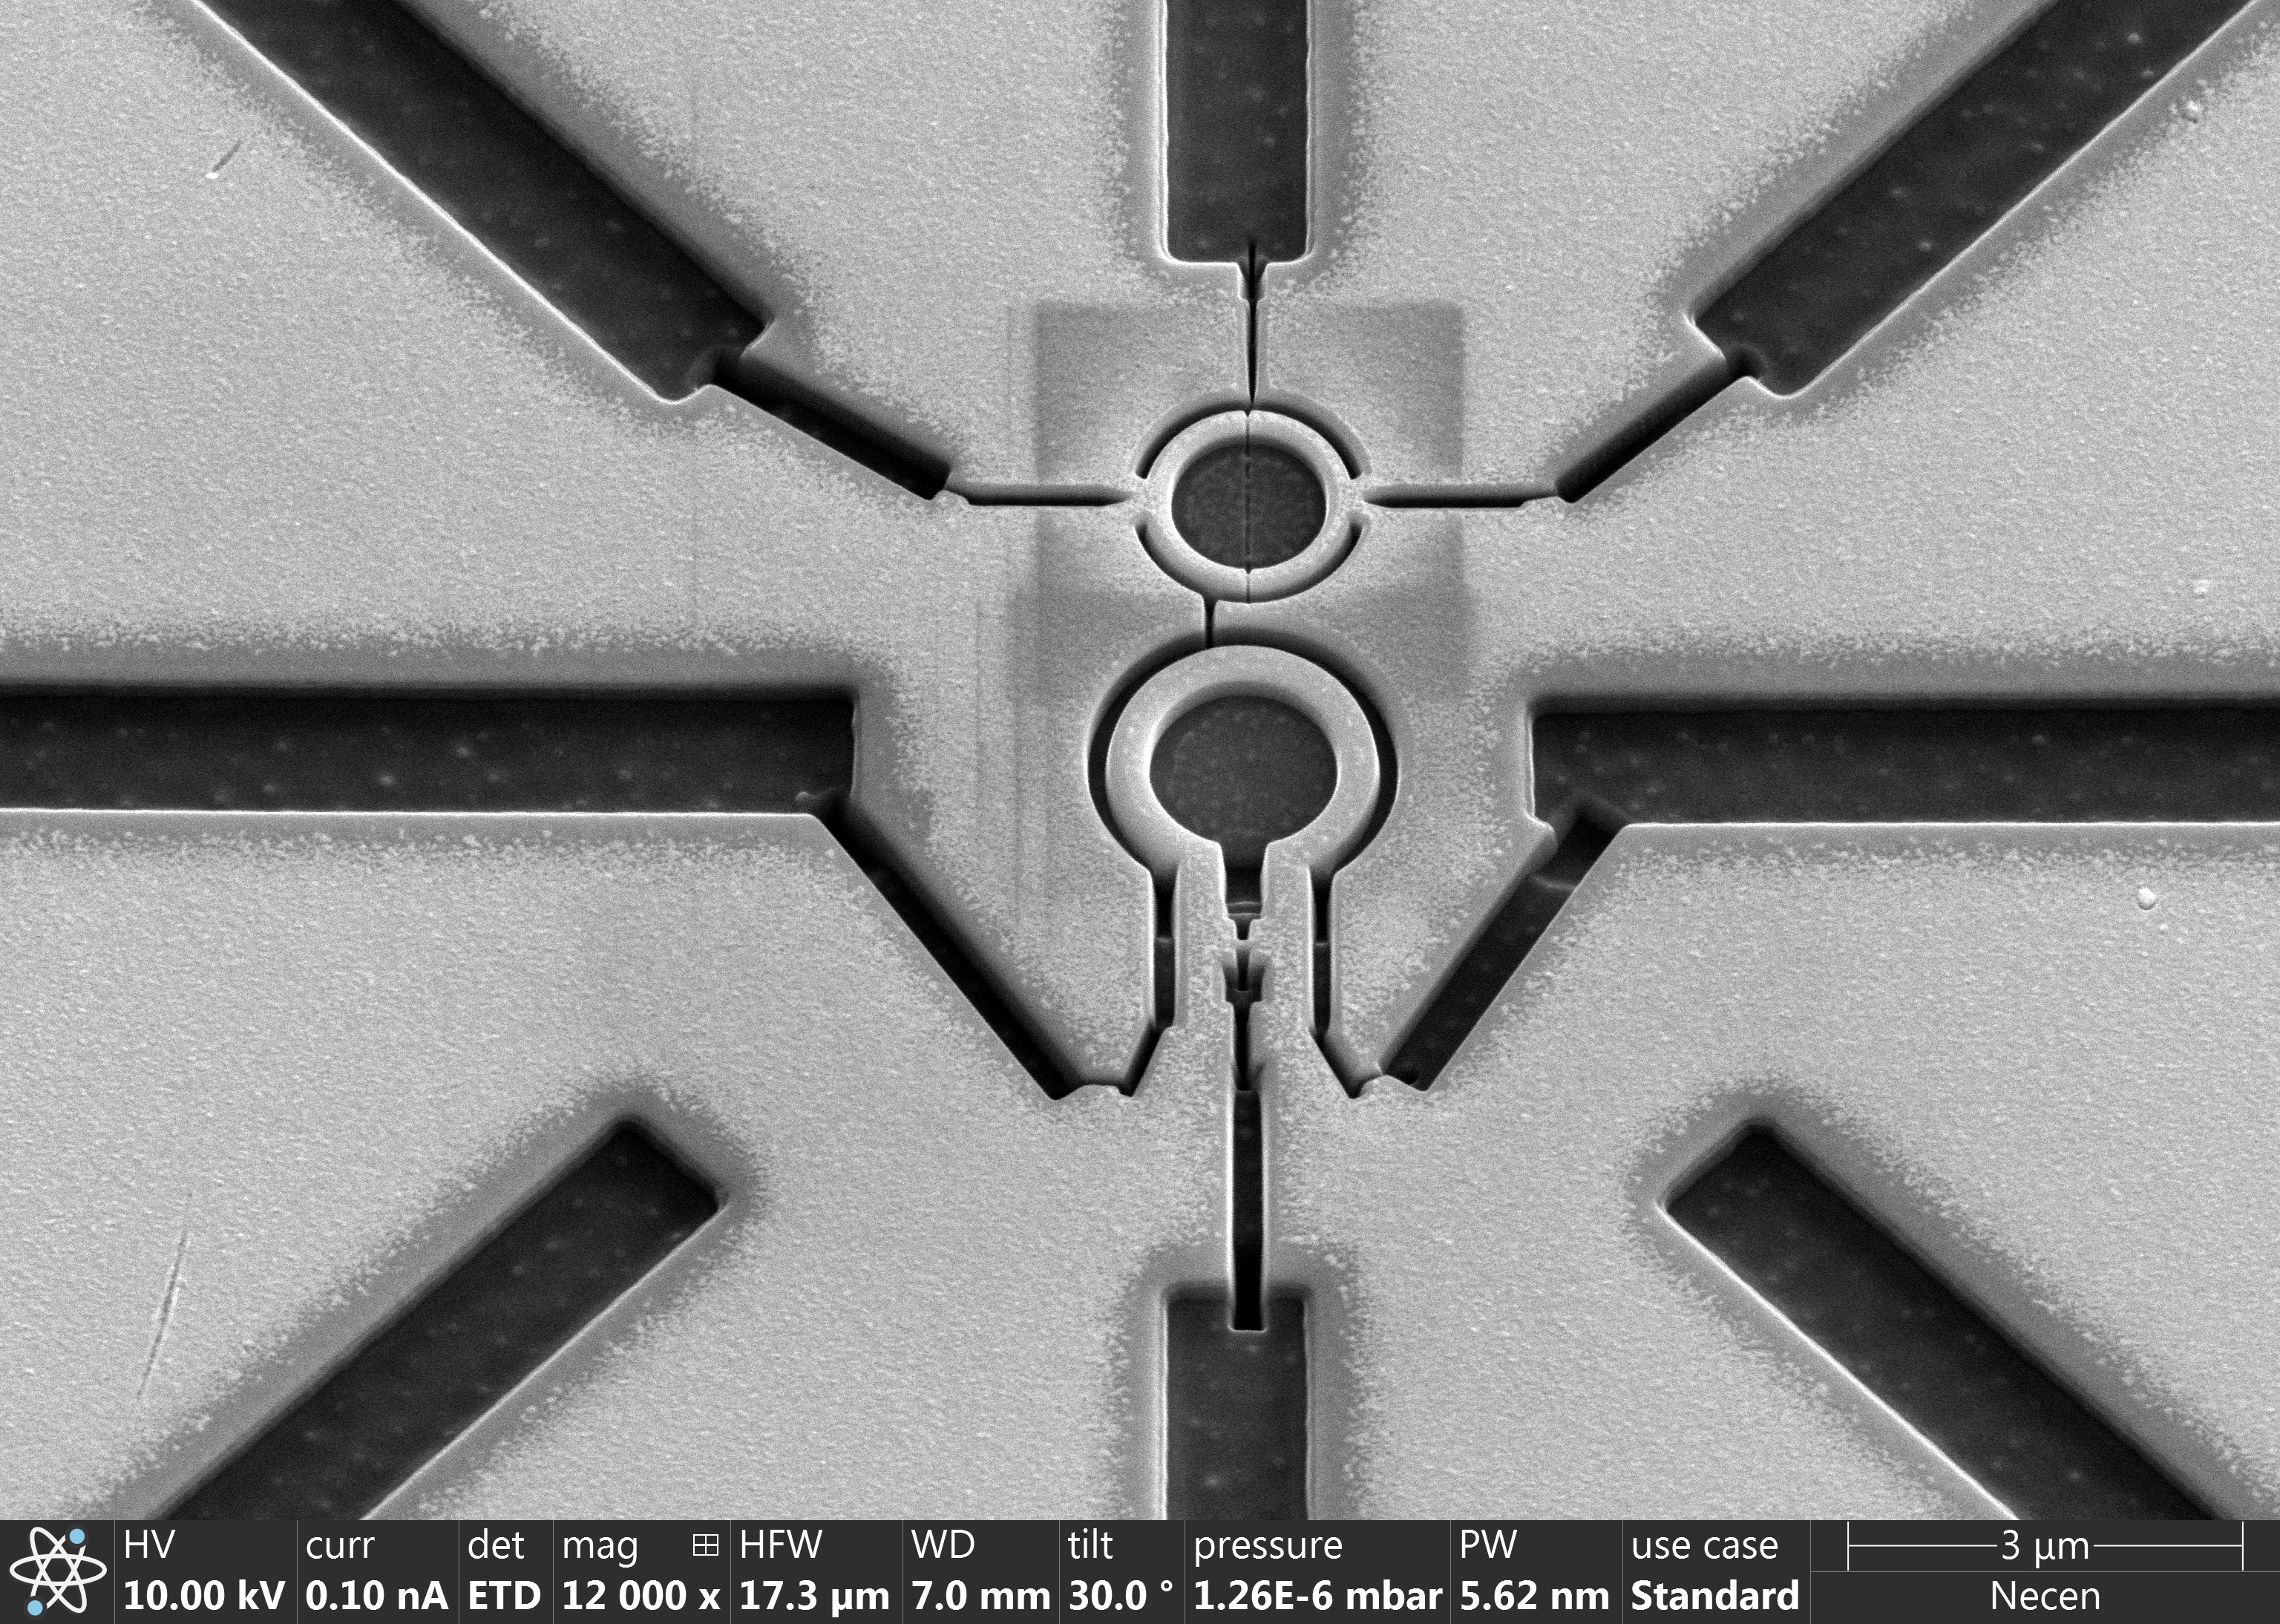
\includegraphics[width=\textwidth]{figures/samples/CP1/CP1.2H_SEM_overview.jpg}
		\subcaption{Overview of the fine structures. On the left we see the junction's loop and on the right the dc-SQUID. The view has been rotated \qty{90}{\degree} clockwise compared to the other figures for visual clarity.}
	\end{subfigure}
	\hfill
	\begin{subfigure}[t]{0.3\textwidth}
		\centering
		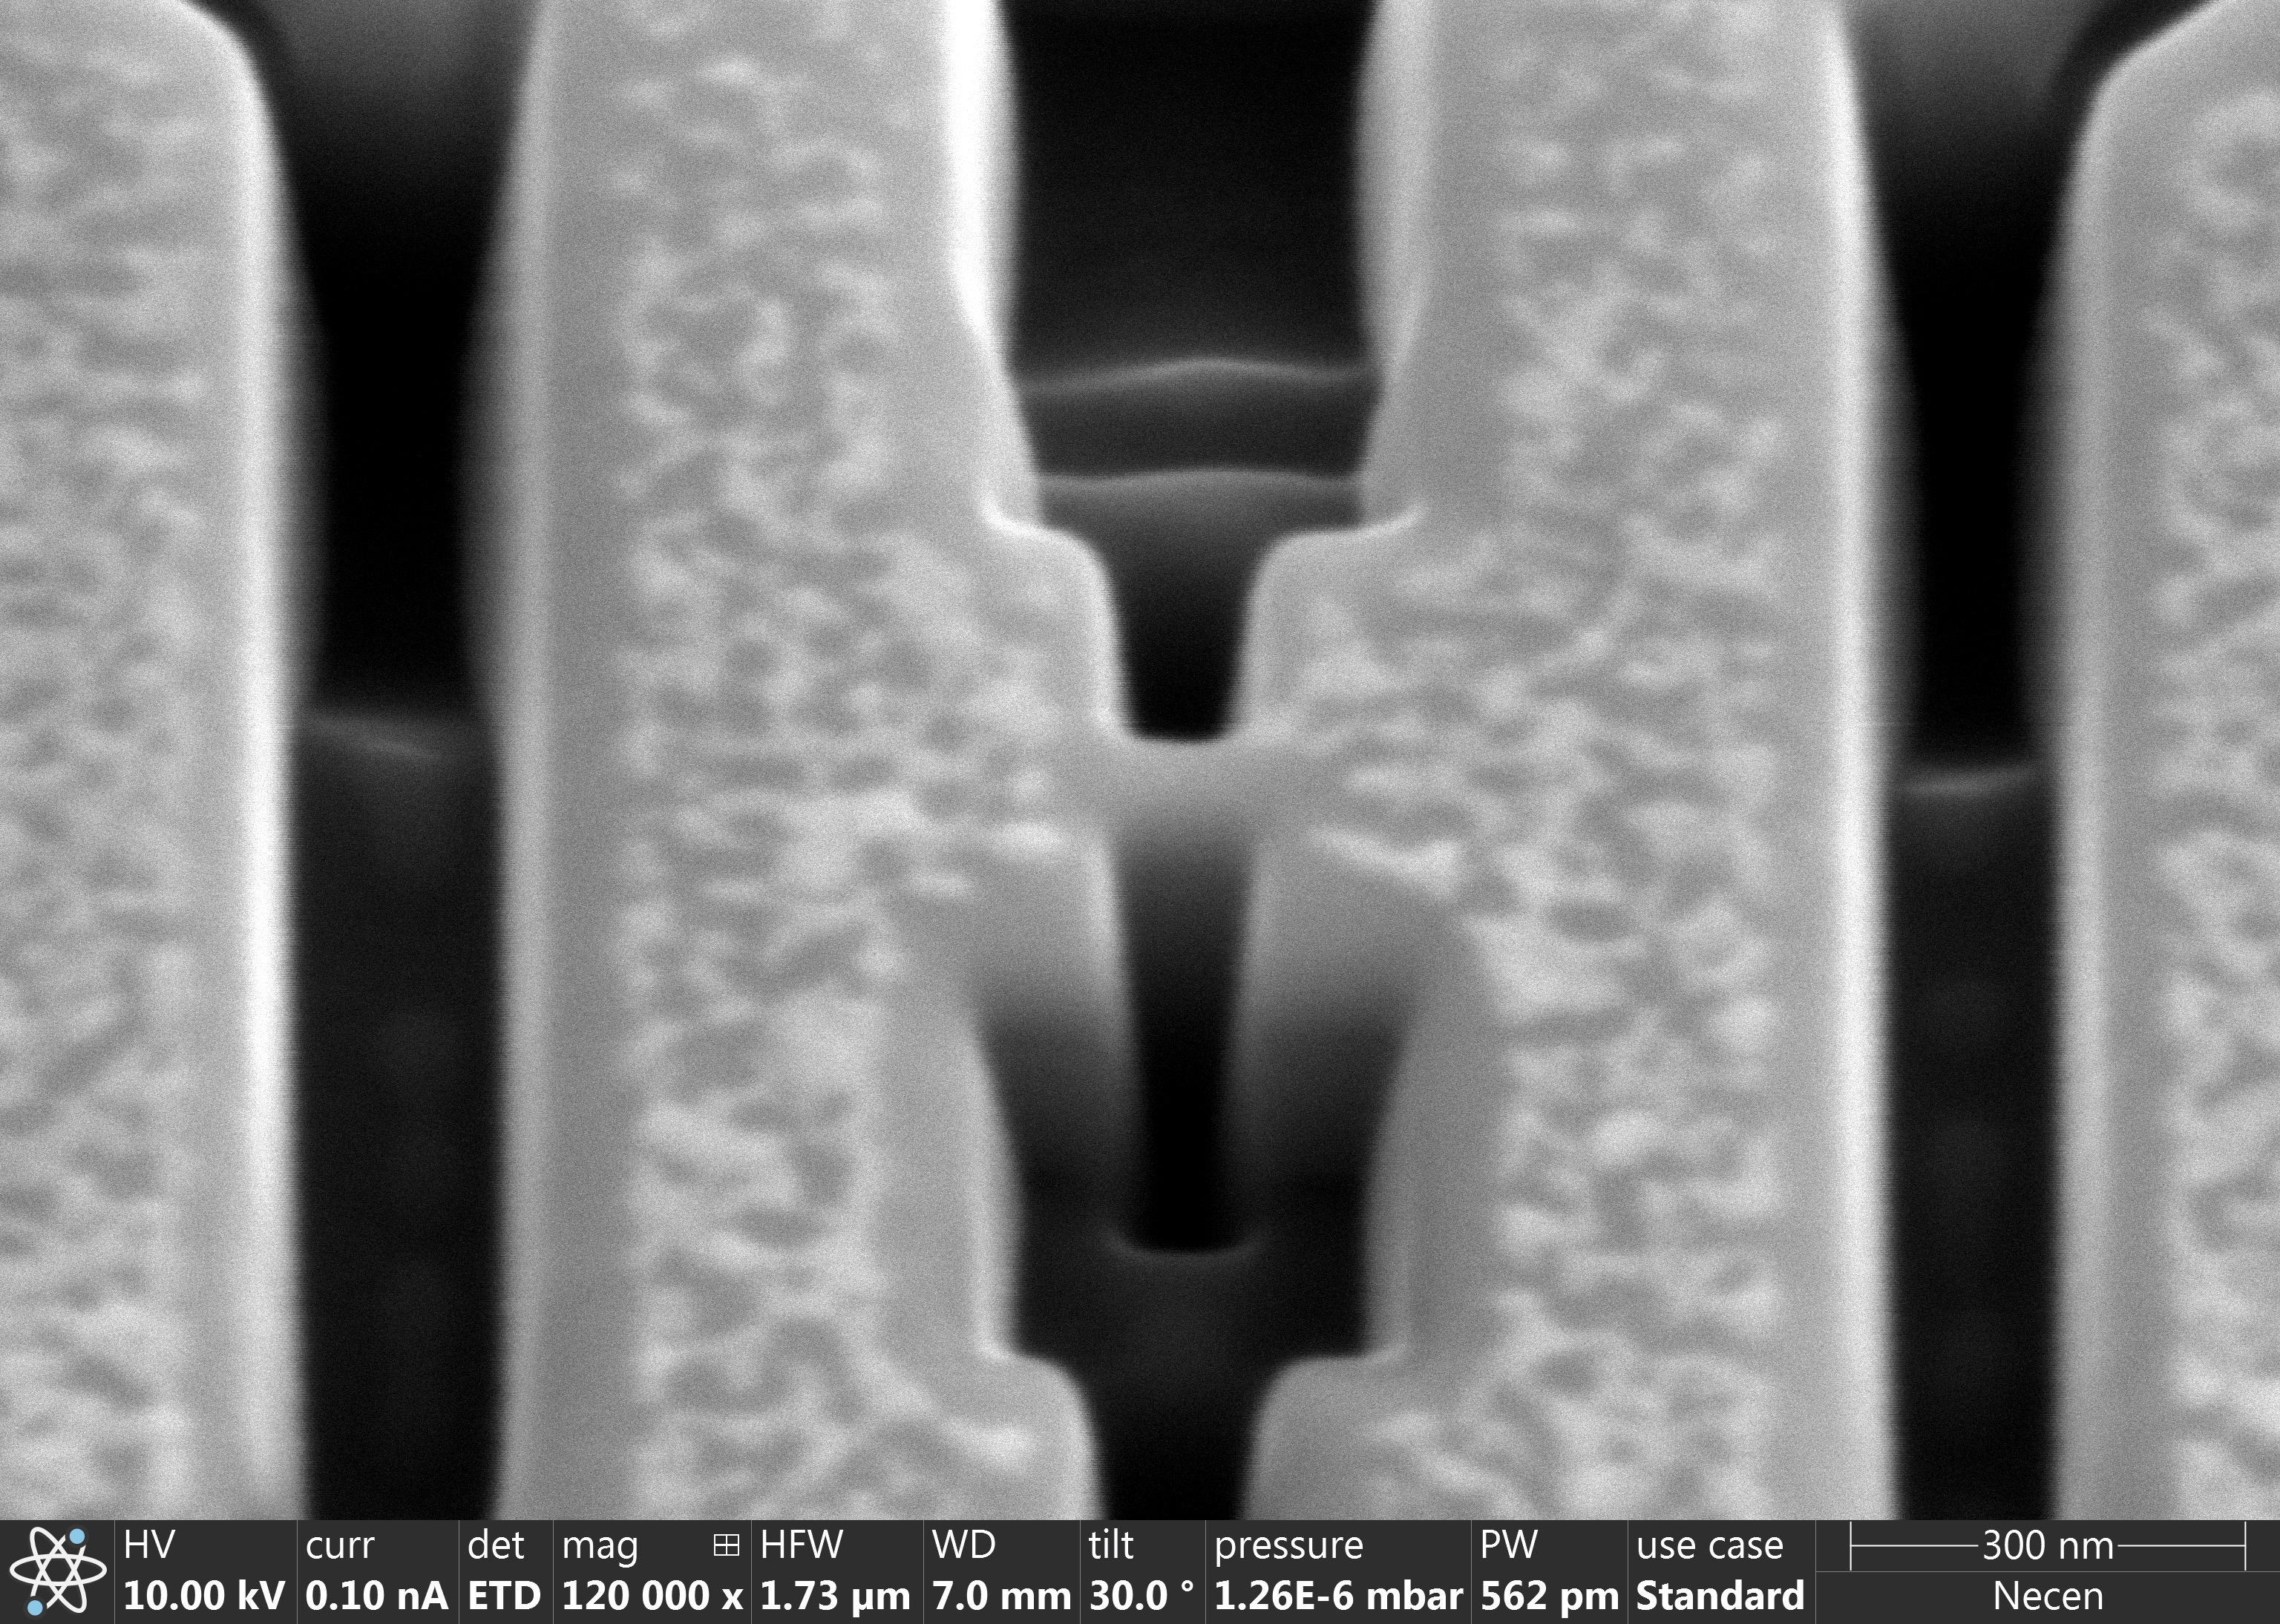
\includegraphics[width=\textwidth]{figures/samples/CP1/CP1.2H_SEM_junction.jpg}
		\subcaption{Zoomed in view of the junction, the size of the junction is \qty{100}{\nano\meter} by \qty{80}{\nano\meter}. The viewing angle is \qty{30}{\degree}.}
	\end{subfigure}
	\hfill
	\begin{subfigure}[t]{0.3\textwidth}
		\centering
		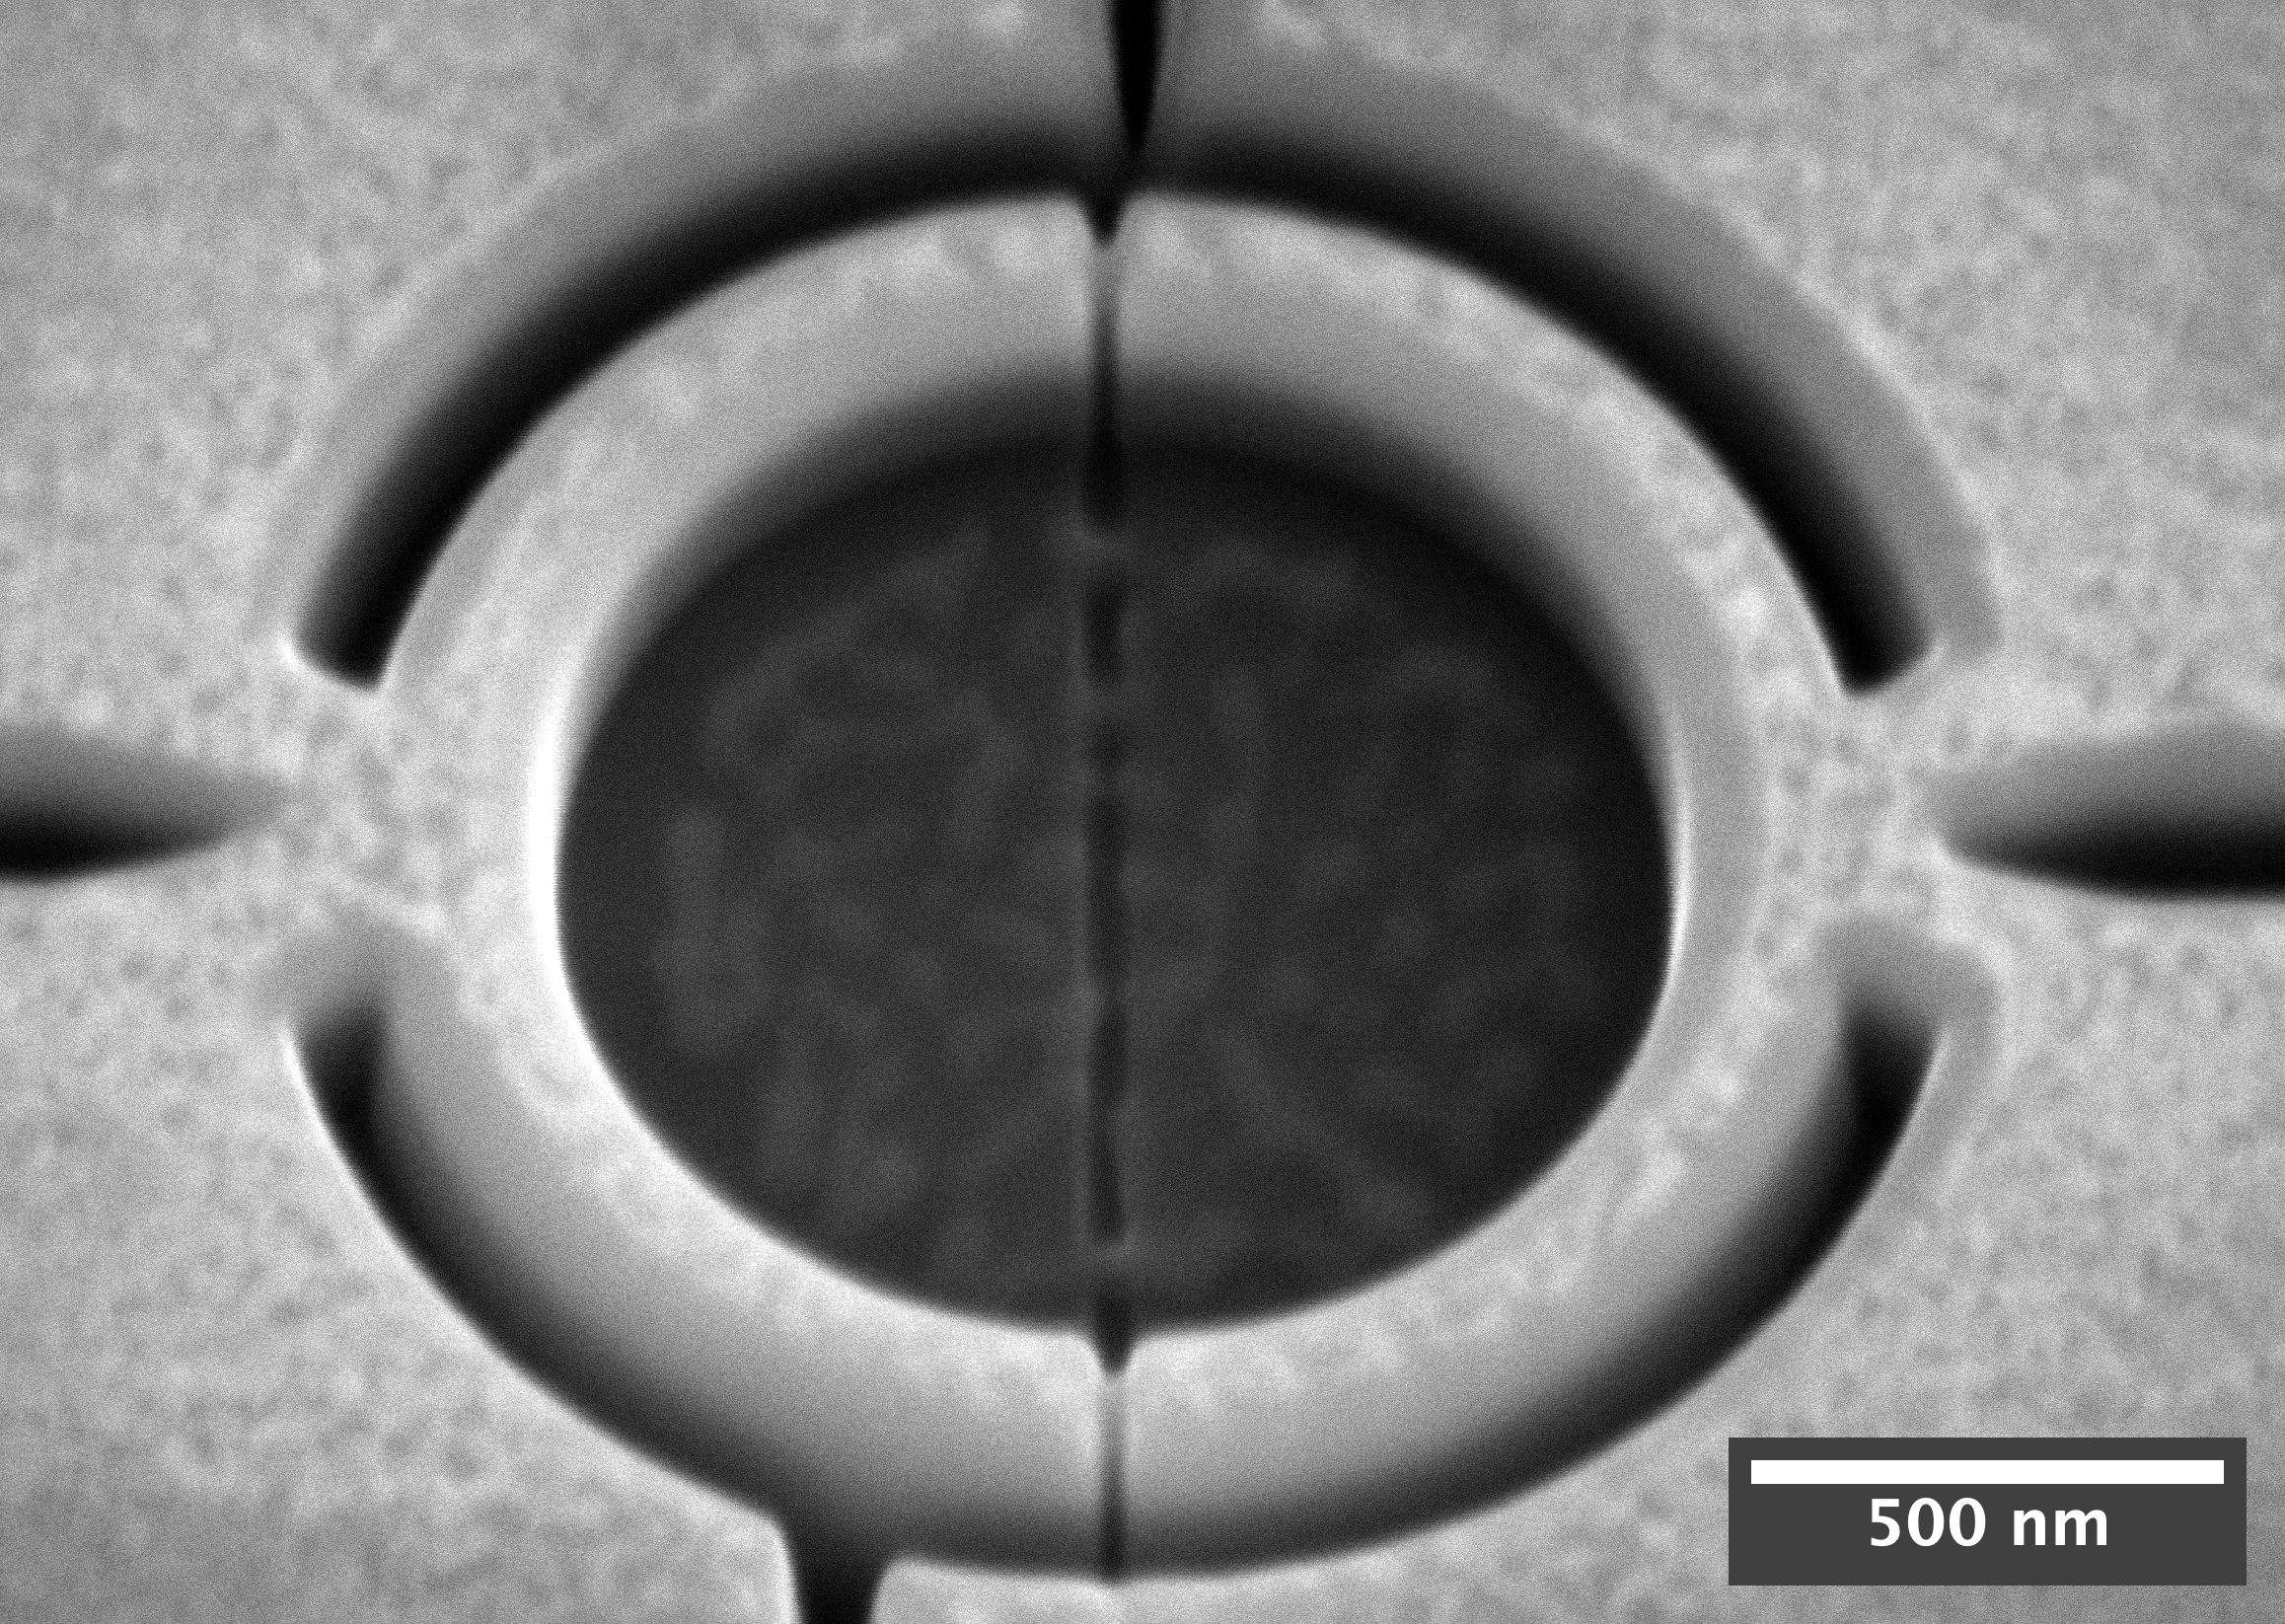
\includegraphics[width=\textwidth]{figures/samples/CP1/CP1.2H_SEM_SQUID.jpg}
		\subcaption{Zoomed in view of the dc-SQUID. The width of the junctions is \qty{19}{\nano\meter}. The viewing angle is \qty{30}{\degree}.}
	\end{subfigure}

	\caption{Fine structures of sample CP1 after the FIB. Table~\ref{tab:CP1.6H-geometries} shows the exact geometries of the sample.}
	\label{fig:CP1.2H-SEM-images}
\end{figure}

\begin{table}
	\begin{subtable}{.6\linewidth}
		\begin{tabular}[t]{@{}lrr@{}}
			\toprule
			Parameter & Value \\ \midrule
			\expandableinput tables/geometries/CP1.2H.tex
			\bottomrule
		\end{tabular}
    \end{subtable}
    \hfill
    \begin{subtable}{.3\linewidth}
    	\flushright
    	\begin{tabular}[t]{@{}lrr@{}}
    		\toprule
    		Parameter & Value \\ \midrule
    		\expandableinput tables/parameters/CP1.2H.tex
    		\bottomrule
    	\end{tabular}
    \end{subtable}
    \caption{The \textbf{left} table provides an overview of the geometries of CP1.6H as determined by SEM imaging and sputtering rates. The \textbf{right} table gives an overview of parameters found using a simulation based on the geometries. The geometries of the dc-SQUID are based on earlier work by \citeauthor{rogSQUIDontipMagneticMicroscopy2022} \citeyear{rogSQUIDontipMagneticMicroscopy2022}.}
    \label{tab:CP1.6H-geometries}
\end{table}